\chapter{Introduction}

\section{Perfect Game of Tic Tac Toe}

To begin, let's start by defining what it means to \emph{play a perfect game of tic tac toe}: \\ 

If I play perfectly, every time I play I will either win the game, or I will draw the game. Furthermore if I play against another perfect player, I will always draw the game. How might we describe these situations quantitatively? Let's assign a score to the "\emph{end game conditions}:"

\begin{itemize}
	\itemsep-0.5em 
	\item I win, hurray! I get 10 points!
    \item I lose, shit. I lose 10 points (because the other player gets 10 points).
    \item I draw, whatever. I get zero points, nobody gets any points.
\end{itemize}

To apply this, let's take an example from near the end of a game, where it is my turn. I am X. My goal here, obviously, is to maximize my end game score.\\

\begin{center}
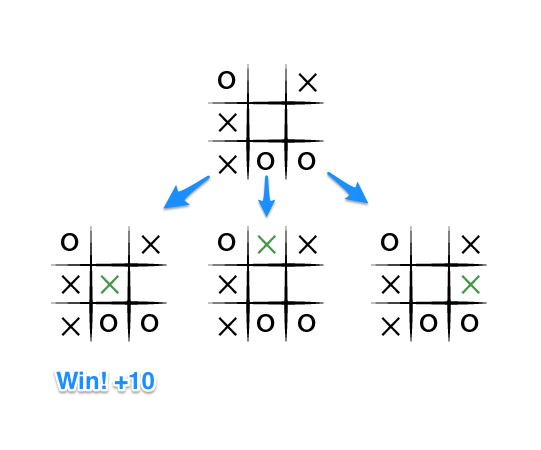
\includegraphics[width=1.1\textwidth]{./a-contrived-end-state-for-a-tic-tac-toe-game}
\end{center}

If the top of this image represents the state of the game I see when it is my turn, then I have some choices to make, there are three places I can play, one of which clearly results in me wining and earning the 10 points. If I don't make that move, O could very easily win. And I don't want O to win, so my goal here, as the first player, should be to pick the maximum scoring move. \\

What do we know about O? Well we should assume that O is also playing to win this game, but relative to us, the first player, O wants obviously wants to chose the move that results in the worst score for us, it wants to pick a move that would minimize our ultimate score. Let's look at things from O's perspective, starting with the two other game states from above in which we don't immediately win: \\

\begin{center}
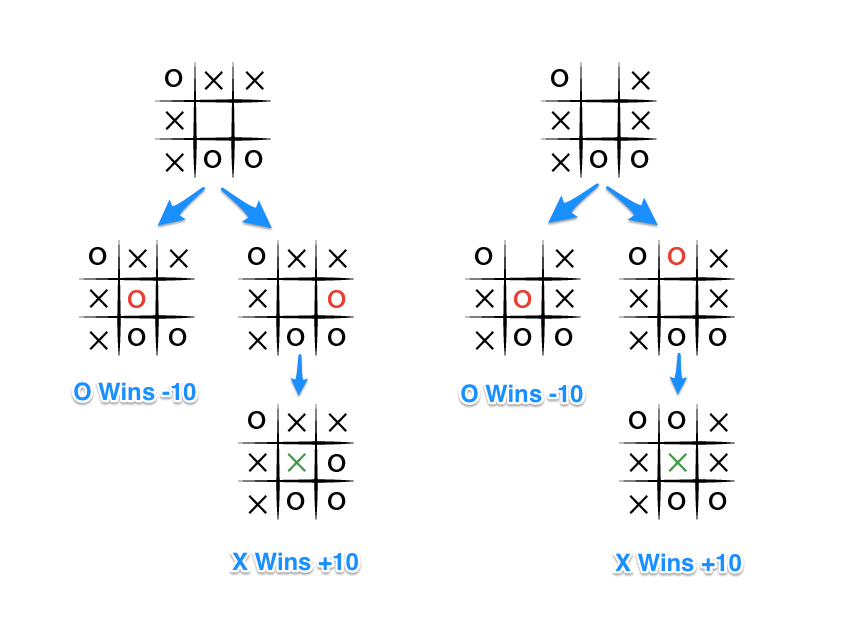
\includegraphics[width=1.1\textwidth]{./a-move-tree-from-the-perspective-of-the-other-player-o}
\end{center}

The choice is clear, O would pick any of the moves that result in a score of -10.

\subsection{Minimax Algorithm}

The key to the Minimax algorithm is a back and forth between the two players, where the player whose "turn it is" desires to pick the move with the maximum score. In turn, the scores for each of the available moves are determined by the opposing player deciding which of its available moves has the minimum score. And the scores for the opposing players moves are again determined by the turn-taking player trying to maximize its score and so on all the way down the move tree to an end state. \\

A description for the algorithm, assuming X is the "turn taking player," would look something like: 

\begin{itemize}
	\itemsep-0.5em 
	\item If the game is over, return the score from X's perspective.
	\item Otherwise get a list of new game states for every possible move.
	\item Create a scores list.
	\item For each of these states add the minimax result of that state to the scores list.
	\item If it's X's turn, return the maximum score from the scores list.
	\item If it's O's turn, return the minimum score from the scores list.
\end{itemize}

\begin{lstlisting}
def minimax(depth, player)
  if gameover || depth == 0
    return calculated_score
  end
  children = all legal moves for player
  if player is AI (maximizing player)
    best_score = -infinity
    for each child
      score = minimax(depth - 1, opponent)
      if (score > best_score)
        best_score = score
      end
      return best_score
    end
  else #player is minimizing player
    best_score = +infinity
    for each child
      score = minimax(depth - 1, player)
      if (score < best_score)
        best_score = score
      end
      return best_score
    end
  end
end

#then you would call it like
minimax(2, computer)
\end{lstlisting}

\begin{center}
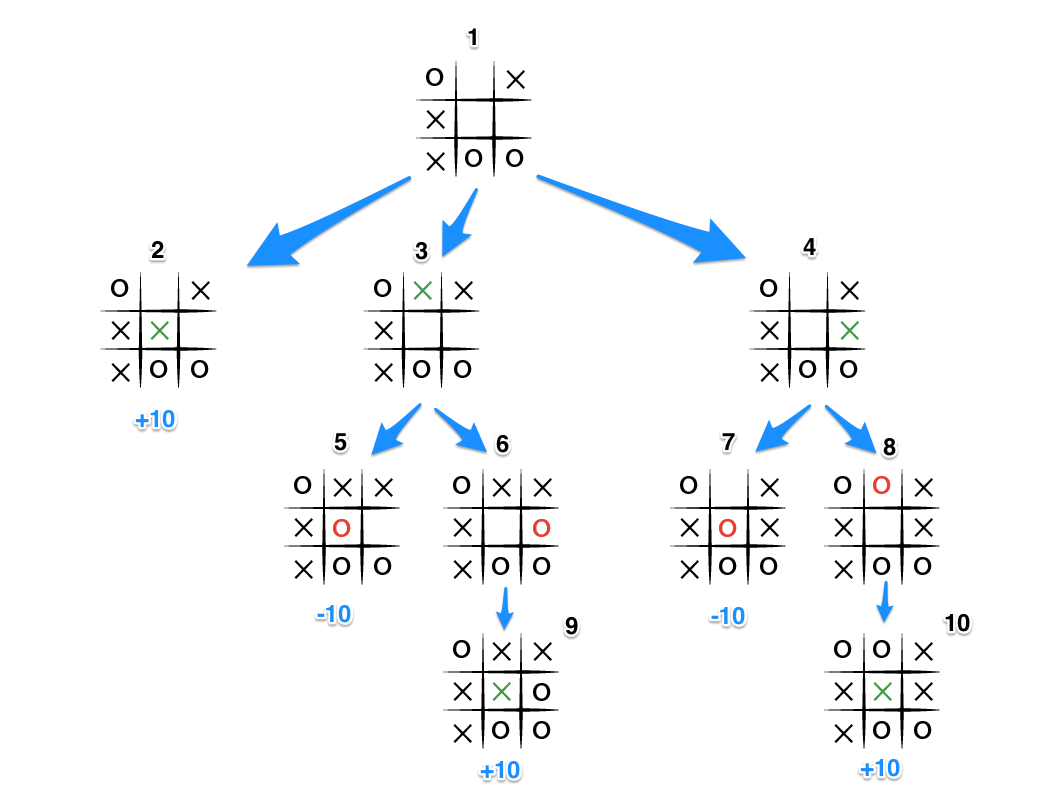
\includegraphics[width=0.9\textwidth]{./full-minimax-move-tree}
\end{center}

\subsection{Alpha-Beta Pruning}

There’s a different algorithm that makes Minimax better, called Alpha-beta pruning. This eliminates paths that are worse than paths that have already been evaluated. Therefore, you have to store a few more values: alpha, which holds the maxmimum score for the maximum path, and beta, which holds the minimum score for the minimum path. You throw away a path when its alpha value is \textgreater= the beta value. \\

\begin{center}
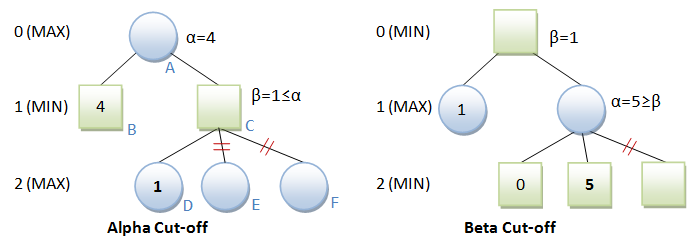
\includegraphics[width=1.1\textwidth]{./GameTTT_alphabeta}
\end{center}

\begin{lstlisting}
def minimax(depth, player, alpha, beta)
  if gameover || depth == 0
    return calculated_score
  end
  children = all legal moves for player
  if player is AI (maximizing player)
    for each child
      score = minimax(depth - 1, opponent, alpha, beta)
      if (score > alpha)		alpha = score	end
      if alpha >= beta     	break			end
      return alpha
    end
  else #player is minimizing player
    best_score = +infinity
    for each child
      score = minimax(depth - 1, player, alpha, beta)
      if (score < beta)		beta = score		end
      if alpha >= beta		break			end
      return beta
    end
  end
end

#then you would call it like
minimax(2, computer, -inf, +inf)
\end{lstlisting}